\documentclass[10pt]{article}
\usepackage[total={6in,9.25in}]{geometry}
\usepackage[utf8]{inputenc}
\usepackage{listings}
\usepackage{hyperref}
\usepackage{graphicx}
\usepackage{amsmath}
\usepackage{amsfonts}
\usepackage{amssymb}
\usepackage{caption}
\usepackage[framed,numbered]{mcode}
\graphicspath{ {./images/} }
\lstset{language=Python}
\author{Jamison Lahman}
\title{Computational Physics: Chapter 1}
\begin{document}

\begin{flushright}Jamison Lahman (\href{mailto:lahmanja@protonmail.com}{lahmanja@protonmail.com}) \\
\href{https://www.amazon.com/Computational-Physics-Fortran-Steven-Koonin/dp/0201386232}{Computational Physics: FORTRAN Version} \\
by Steven E. Koonin and Dawn C. Meredith\\
Chapter 01 Exercises | July 7th, 2018 \\
\end{flushright}
\label{exercise:1.1}\textbf{Exercise 1.1:} Using any function for which you can evaluate the derivatives analytically, investigate the accuracy of the formulas in Table 1\footnote{Table 1.2 from \href{https://www.amazon.com/Computational-Physics-Fortran-Steven-Koonin/dp/0201386232}{Computational Physics: FORTRAN Version}} for various values of \textit{h}. \\
\\
\label{summary:1.1}\textbf{Summary:} To approximate the derivative numerically, we will utilize five equations based off the Maclaurin Series. The Maclaurin Series of function, \textit{f(x)}, is given by the equation,

\begin{equation}
	f(x) = f_0 +x f_0'+ \frac{x^2f_0''}{2!} + \frac{x^nf_0^{n}}{n!}.
\end{equation}
Solving the above equation for \textit{f'} yields,

\begin{equation}
	f_0' = \frac{f(x)-f_0}{x}+\frac{-1}{x}\left(\frac{x^2f_0''}{2!} \right)+ \frac{-1}{x} \left(\frac{x^nf_0^{(n)}}{n!}\right) =  \frac{f(x)-f_0}{x}  + \mathcal{O}(x).
\end{equation}
The above equation assumes the function is accurately described by a linear function over the interval $(0,h)$. This gives the first of the "2-point" methods, the forward 2-point method,

\begin{equation}
\label{eq:forward2}
	f'(x) \approx \frac{f(x_{k+1})-f(x_k)}{h},
\end{equation}
where \textit{x} is the value where the derivative is being evaluated and \textit{h} is the step size used. Using the same method as above but using a previous point produces the equation,

\begin{equation}
\label{eq:backward2}
	f'(x) \approx \frac{f(x_k)-f(x_{k-1})}{h}.
\end{equation}
This assumes the function is accurately described by a linear function over the interval $(-h,0)$. Notice each of these equations are accurate up to one order of \textit{h}. The following are python functions utilizing each respective 2-point method,
\begin{lstlisting}
def forward2(x,h):
#Performs the forward 2-point method on the function defined by myFunc
#Input:  x -- independent variable
#        h -- step-size
#Output: dependent variable
    return((myFunc(x)-myFunc(x-h))/h)

def backward2(x,h):
#Performs the backward 2-point method on the function defined by myFunc
#Input:  x -- independent variable
#        h -- step-size
#Output: dependent variable
    return((myFunc(x+h)-myFunc(x))/h)
\end{lstlisting}

We can improve the accuracy by including more terms. Using the immediate values forwards and backwards allows for the terms with even-powered values of \textit{h} to cancel out. Eq \ref{eq:symmetric3} is the quadratic polynomial interpolation of the function over the two previous regions,

\begin{equation}
\label{eq:symmetric3}
	f'=\frac{f(x_{k+1})-f(x_{k-1})}{2h} + \mathcal{O}(h^2).
\end{equation}
Python interpration of Eq.\ref{eq:symmetric3},
\begin{lstlisting}
def symmetric3(x,h):
#Performs the symmetric 3-point method on the function defined by myFunc
#Input:  x -- independent variable
#        h -- step-size
#Output: dependent variable
    return((myFunc(x+h) - myFunc(x-h)) / (2*h))
\end{lstlisting}

The final two equations, the "4-point" and "5-point" formulas, are similarly found and include more interactions fowards and backwards to create higher-order approximations of the function over the given interval. They, along with their higher-order derivatives, are given in Table \ref{tab:differentiation}. The 5-point formula is the five-point stencil in one-dimension. \\
\begin{table}[!ht]
	% Center the table
	\begin{center}
    % Title of the table
	\caption{4- and 5-point difference formulas for derivatives}
		\label{tab:differentiation}
		\begin{tabular}{|ccc|}
		% To create a horizontal line, type \hline
		\hline
		& 4-point & 5-point \\
		\hline
		$hf'$ & $\pm\frac{1}{6}(-2f_{\mp1} - 3f_{0} + 6f_{\pm 1} - f_{\pm 2})$ & $\frac{1}{12}(f_{-2} - 8f_{-1} + 8f_{1} -f_{2})$ \\
		$h^{2}f'' $ & $f_{-1} - 2f_{0} + f_{1}$ & $\frac{1}{12}(-f_{-2}+16f_{-1} - 30 f_{0} +16f_{1} -f_{2})$ \\
		$h^{3}f'''$ & $\pm(-f_{\mp 1} + 3 f_{0} - 3 f_{\pm 1} + f_{\pm 2 })$ & $\frac{1}{2}(-f_{-2} + 2f_{-1} - 2f_{1} + f_{2})$ \\
		$h^{4}f^{iv)} $ & ... & $f_{-2} - 4 f_{-1} + 6 f_{0} -4f_{1} + f_{2}$ \\
		\hline
		\end{tabular}
	\end{center}
\end{table} \\
Python interpretation of the previous equations,

\begin{lstlisting}
def symmetric4(x,h):
#Performs the symmetric 4-point method on the function defined by myFunc
#Input:  x -- independent variable
#        h -- step-size
#Output: dependent variable
    return((-2*myFunc(x-h)-3*myFunc(x)+6*myFunc(x+h)-myFunc(x+2*h))/(6*h))

def symmetric5(x,h):
#Performs the symmetric 5-point method on the function defined by myFunc
#Input:  x -- independent variable
#        h -- step-size
#Output: dependent variable
    return((myFunc(x-2*h)-8*myFunc(x-h)+8*myFunc(x+h)-myFunc(x+2*h))/(12*h))
\end{lstlisting}
\label{solution:1.1}\textbf{Solution:}
\begin{table}[!ht]
	% Center the table
	\begin{center}
    % Title of the table
	\caption{Error in evaluating the $d \sin /dx|_{x=1}=0.540302$}
		\label{tab:diff_errors}
		\begin{tabular}{|cccccc|}
		% To create a horizontal line, type \hline
		\hline
		h & Fwd 2-pnt Eq. \ref{eq:forward2} & Bkwd 2-pnt Eq. \ref{eq:backward2} & 3-pnt Eq. \ref{eq:symmetric3} & 4-pnt Tab. \ref{tab:differentiation} & 5-pnt Tab. \ref{tab:differentiation} \\
		\hline
		0.50000&-0.228254&0.183789&-0.022233&-0.009499&-0.001093\\
		0.20000&-0.087462&0.080272&-0.003595&-0.000586&-0.000029\\
		0.10000&-0.042939&0.041138&-0.000900&-0.000072&-0.000002\\
		0.05000&-0.021257&0.020807&-0.000225&-0.000009&-0.000000\\
		0.02000&-0.008450&0.008378&-0.000036&-0.000001&-0.000000\\
		0.01000&-0.004216&0.004198&-0.000009&-0.000000&-0.000000\\
		0.00500&-0.002106&0.002101&-0.000002&-0.000000&-0.000000\\
		0.00200&-0.000842&0.000841&-0.000000&-0.000000&-0.000000\\
		0.00100&-0.000421&0.000421&-0.000000&-0.000000&-0.000000\\
		0.00050&-0.000210&0.000210&-0.000000&-0.000000&-0.000000\\
		0.00020&-0.000084&0.000084&-0.000000&-0.000000&-0.000000\\
		0.00010&-0.000042&0.000042&-0.000000&0.000000&0.000000\\
		0.00005&-0.000021&0.000021&-0.000000&0.000000&0.000000\\
		0.00002&-0.000008&0.000008&-0.000000&-0.000000&0.000000\\
		0.00001&-0.000004&0.000004&-0.000000&-0.000000&-0.000000\\
		\hline
		\end{tabular}
	\end{center}
\end{table}
The function we will approximating the derivative numerically is,

\[
	F(x) = \sin(x).
\]
The analytical derivative of the sine function is known to be,

\[
	\frac{d \sin(x)}{dx} = \cos(x).
\]
For a formal proof of the derivation, see \href{https://en.wikipedia.org/wiki/Differentiation_of_trigonometric_functions#Derivative_of_the_sine_function}{Wikipedia - derivative of the sine function}. The exact value of the derivative at $x=1$ (up to six decimal points) is $0.540302$. Table \ref{tab:diff_errors} shows the accuracy of the formulas above for various values of \textit{h}.\footnote{For the full program responsible for Table \ref{tab:diff_errors}, see my \href{https://github.com/jmelahman/computational-physics-solutions/blob/master/exercises_python/Chapter\%201/exercise1_1.py}{GitHub}.} \\

\newpage\noindent\label{exercise:1.2}\textbf{Exercise 1.2:} Using any function whose definite integral you can compute analytically, investigate the accuracy of various quadrature methods for various values of \textit{h}. \\
\\
\label{summary:1.2}\textbf{Summary:}
To approximate the definite integral of a function over the interval [\textit{a,b}], we will employ similar methods as used previously for exercise 1.1. A simple approximation is to assume the function is linear over the entire interval (see the star-dashes in Fig.\ref{fig:interpolation}). Further accuracy can be found by splitting the interval into N number of smaller lattices which can then be approximated linearly,

\[
	N = \frac{b-a}{h},
\]
where \textit{h} is the width of the lattice (see the dashed lines in Fig.\ref{fig:interpolation}). The integral is then,

\begin{equation}
	\label{eq:trapezoidal}
	\int^b_a f(x)dx = \sum^N_{k=1} \frac{h}{2}[f(x_{k-1})+f(x_k)] + \mathcal{O}(h^3) \approx T_N.
\end{equation}

\begin{figure}[!ht]
	% Center the figure.
    \begin{center}
	% Include the eps file, scale it such that it's width equals the column width. You can also put width=8cm for example...
	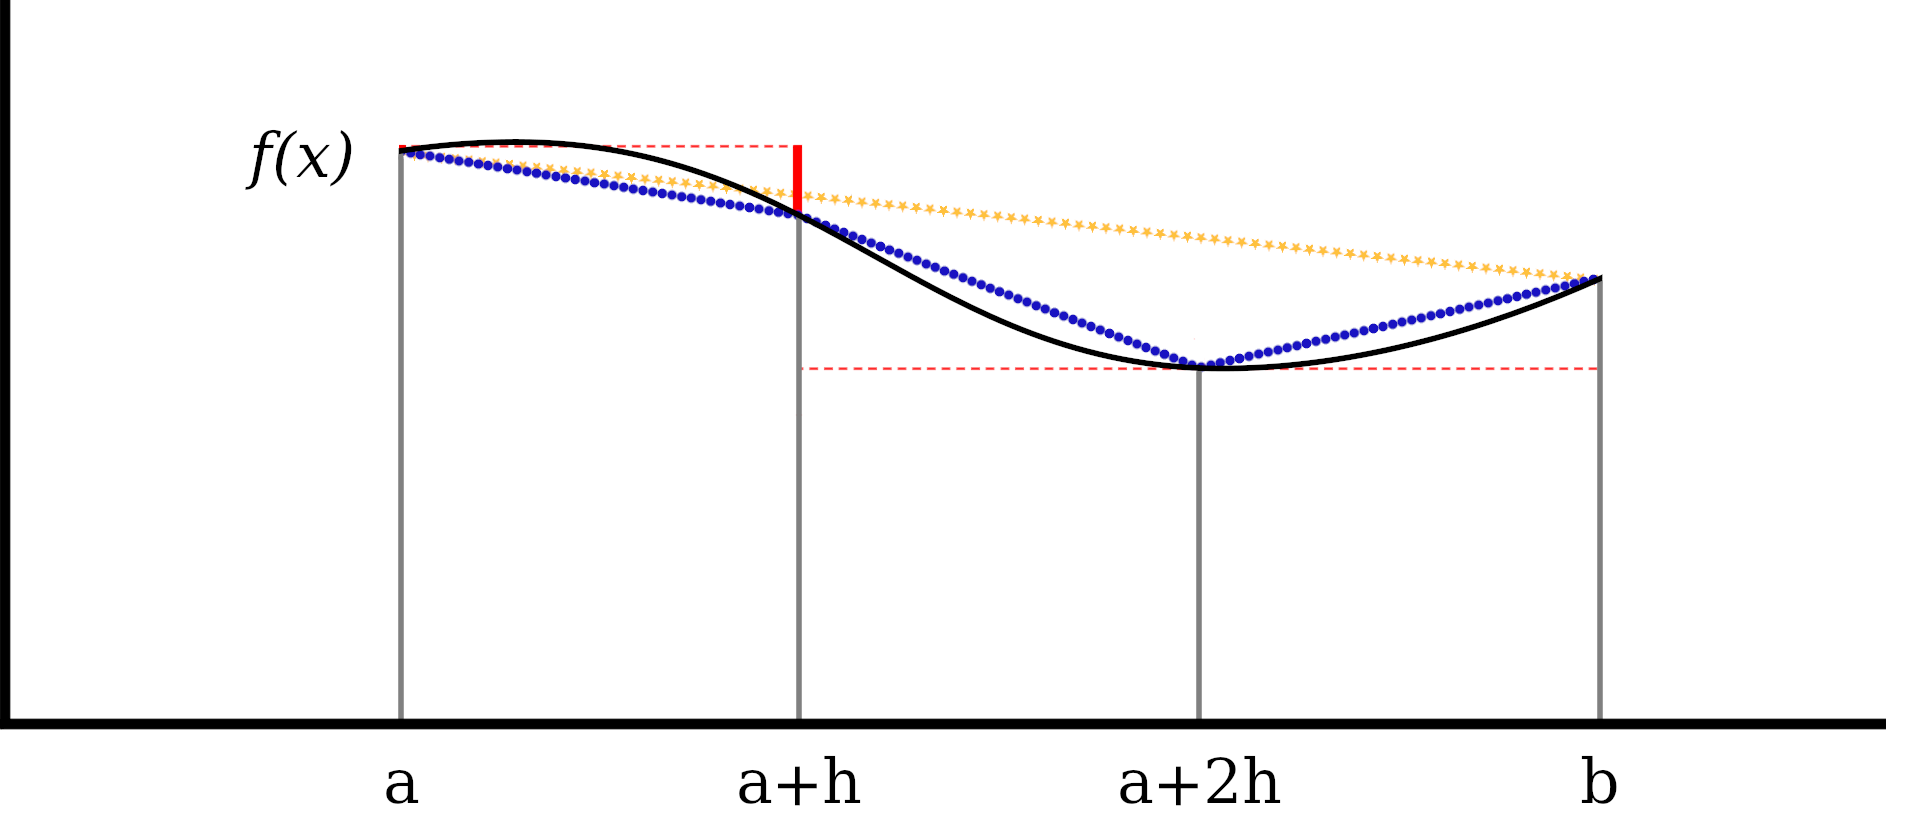
\includegraphics[width=\columnwidth]{interpolation.png}
	% Create a subtitle for the figure.
	\caption{The yellow, star-dashed line show shows a linear interpolation of the function over the full domain. The blue, circle-dashed line shows a linear interpolation of the function with lattices of width \textit{h}. The red, dashed line shows the midpoint method. It is easy to see the trapezoid method over-estimates the integral over the interval [\textit{a+h,b}] whereas the midpoint method under-estimates.}
	% Define the label of the figure. It's good to use 'fig:title', so you know that the label belongs to a figure.
	\label{fig:interpolation}
	\end{center}
\end{figure}

The Python interpretation of the Trapezoid method is,
\begin{lstlisting}
def trapezoidal(myFunc,x,h,N):
#Performs the trapezoidal rule (equation 1.9). The average of the function evaluated at
#the end points of the lattice multiplied by the change in the independent variable.
#Input:  x -- lower bound of the range of integration
#        h -- step-size
#        N -- number of lattices
#Output: ans -- approximate integral
#JL TODO: This evaluates myFunc twice at x+(i+1)*h then again at x+i_{+}*h. Could be improved
#to use results from previous iteration.
    return(sum((myFunc(x+i*h)+myFunc(x+(i+1)*h))*h/2.0 for i in range(N)))
\end{lstlisting}

The behavior of the error for the trapezoid method is very much dependent on the behavior of the function over the given interval. When the function is concave up (such as the the function over the interval [\textit{a+h,b}] in Fig.\ref{fig:interpolation}), the trapezoid method will over-estimate the true value. Similarly, when the function is concave down, (such as the function over the interval [\textit{a,a+h}] in Fig.\ref{fig:interpolation}), the trapezoid method will under-estimate the true value.

Conversely, the midpoint method,

\begin{equation}
	\label{eq:midpoint}
	\int^b_a f(x)dx = \sum^N_{k=1} h\cdot f\left(\frac{x_{k-1}+x_k}{2}\right) + \mathcal{O}(h^3) \approx M_N,
\end{equation}
will consistently approximate in the integral in the opposite direction from the trapezoid method. Given they both error in opposite directions, they can be combined in a manner that reduces the overall error. To be exact, the errors $EM_N$ and $ET_N$ for a quadratic function are related by,

\[
	|EM_N| = \frac{1}{2}|ET_N|
\]
and can be easily combined in a way to completely eliminate this error.\footnote{Taken from Introduction to Numerical Methods and \textsc{matlab} Programming for Engineers by Todd Young and Martin J. Mohlenkamp} This equation is known as the Simpson's Rule,

\[
	S_{2N} = \frac{1}{3}(2M_N + M_N).
\]
Note, in the equation above, S is given the subscript $_{2N}$ since the midpoint is evaluated sub interval points from the trapezoid method thus the number of intervals is twice that for either method. For evenly spaced lattices over the interval [a,b], Simpson's Rule becomes,

\begin{equation}
	\label{eq:simpson}
	S_N = \frac{h}{3}[f(x_k)+4f(x_{k+1})+2f(x_{k+2})+...+2f(x_{n-2})+4f(x_{n-1})+f(x_n)] + \mathcal{O}(h^5).
\end{equation}

The Python interpretation of Simpson's Rule is,
\begin{lstlisting}
def simpsons(myFunc,x,h,N):
#Performs Simpons rule (equation 1.12).
#Input:  x -- lower bound of the range of integration
#        h -- step-size
#        N -- number of lattices
#Output: sum -- approximate integral

#Add the contribution from the first and last points of the domain
    sum = myFunc(x) + myFunc(x+N*h)
    for i in range(1,N):                        #1,N-1 ignores first and last points
#Adds the contribution from the even placed lattice points
        if(i%2 == 1):
            sum = sum+4.0*myFunc(x+i*h)
#Adds the contribution from the odd placed lattice points
        else: sum=sum+2.0*myFunc(x+i*h)
    return(sum *h/3.0)                         #Apply leading factor
\end{lstlisting}

Simpson's Rule is the quadratic interpolation of the function. Similar to numerical differentiation, further accuracy can be achieved by interpolating with higher-order polynomials. The Simpson's 3/8 Rule is the cubic interpolation and is given by,

\begin{equation}
	\label{eq:simpson3/8}
	\int^b_a f(x)dx = \frac{3h}{8}[f(x_k)+3\sum^{N-1}_{i\neq 3j} f(x_i) + 2\sum^{N/3-1}_{j=1} (f(x_{3j})+f(x_n)] + \mathcal{O}(h^5).
\end{equation}
Notice the Simpson's 3/8 Rule accurate to the same order of $h$ as Eq.\ref{eq:simpson} however the constant term is slightly smaller. The quartic interpolation is called Boole's Rule and is given by,

\begin{equation}
	\label{eq:boole}
	\int^b_a f(x)dx = \frac{2h}{45}[ 7f(x_k)+32f(x_{k+1})+12f(x_{k+2})+32f(x_{n-1})+7f(x_n)] + \mathcal{O}(h^7)
\end{equation}

\begin{lstlisting}
def booles(myFunc,x,h,N):
#Performs Bode's rule (equation 1.13b)
#Input:  x -- lower bound of the range of integration
#        h -- step-size
#        N -- number of lattices
#Output: sum -- approximate integral
#Add the contribution from the first and last points of the domain
    sum = 7.0*(myFunc(x)+myFunc(x+N*h))
    for i in range(1,N):                        #N-1 ignores last point
#Adds the contribution from the even placed lattice points
        if(i%2 == 1):
            sum = sum+32.0*myFunc(x+i*h)
        elif(i%4 == 2):
            sum = sum+12.0*myFunc(x+i*h)
#Adds the contribution from the odd placed lattice points
        else: sum = sum+14.0*myFunc(x+i*h)
    return(sum*2.0*h/45.0                  #Apply leading factor
\end{lstlisting}
\label{solution:1.2}\textbf{Solution:}
Using the functions from above, we are able to produce the values for Table \ref{tab:quad_errors}. As we expected, Boole's Rule gives the greatest accuracy with largest value of \textit{h} followed by Simpson's Rule then the Trapezoidal Method.\footnote{For the full program responsible for Table \ref{tab:diff_errors}, see my \href{https://github.com/jmelahman/computational-physics-solutions/blob/master/exercises_python/Chapter\%201/exercise1_2.py}{GitHub}.}
\begin{table}[!ht]
	% Center the table
	\begin{center}
    % Title of the table
	\caption{Errors in evaluating $\int^1_0 e^x dx = 1.718282$ }
		\label{tab:quad_errors}
		\begin{tabular}{|ccccc|}
		% To create a horizontal line, type \hline
		\hline
		N & \textit{h} & Trapezoidal Eq.\ref{eq:trapezoidal} & Simpson's Eq.\ref{eq:simpson} & Boole's Eq\ref{eq:boole} \\
		\hline
		4.000000&0.25000&0.008940&0.000037&0.000001\\
		8.000000&0.12500&0.002237&0.000002&0.000000\\
		16.000000&0.06250&0.000559&0.000000&0.000000\\
		32.000000&0.03125&0.000140&0.000000&0.000000\\
		64.000000&0.01562&0.000035&0.000000&0.000000\\
		128.000000&0.00781&0.000009&0.000000&-0.000000\\
		\hline
		\end{tabular}
	\end{center}
\end{table}

\newpage\noindent
\label{exercise:1.3}\textbf{Exercise 1.3:} Write a program to calculate
\[
\int^1_0 t^{-2/3}(1-t)^{-1/3}dt=2\pi /3^{1/2}
\]
using one of the quadrature formulas discussed above and investigate its accuracy for various values of \textit{h}. (Hint: Split the range of integration into two parts and make a different change of variable in each integral to handle the singularities.\\

\noindent\textbf{Summary:} The equation above has two integrable singularities at \textit{x = 0} where $t^{-2/3}$ is undefined and one at \textit{x = 1} where $(1-t)^{-1/3}$ is undefined. As the hint suggests, the easiest method will be to split the range of integration to isolate each singularity and to perform a separate change of variable to properly approximate.

First, we split the range of integration. Given,
\[
\int^b_a f(x)dx = \int^h_a f(x)dx + \int^b_h f(x)dx,
\]
we can split the integral above into,
\begin{equation}
\int^1_0 t^{-2/3}(1-t)^{-1/3}dt=\int_0^{0.5}t^{-2/3}(1-t)^{-1/3}dt+\int_{0.5}^1t^{-2/3}(1-t)^{-1/3}dt.
\end{equation}
Splitting the integral at 0.5 here was arbitrary and could have realistically been anywhere in the range at least \textit{h} from the endpoints.
From here, we can perform a \textit{u}-substitution inside each integral to handle the singularities. For the first integrand,

\end{document}
